\documentclass[crop=false, class=book]{standalone}

\begin{document}
		
	\subsection{Metodi MGSE, GenomeScope, GCE e findGSE}
	I dati e le figure della seguente analisi sono state ricavate da \cite{pucker2019MGSE}, che esegue un confronto tra i metodi MGSE, GenomeScope, GCE e findGSE. 
	
	Dopo una comparazione iniziale processando due diversi ecotipi di \textit{Arabidopsis thaliana}, i programmi vengono utilizzati per la stima della dimensione di genomi con grandezze e complessità maggiori, come le specie \textit{Beta vulgaris}, \textit{Brachypodium distachyon}, \textit{Solanum lycopersicum}, \textit{Zea mays} e \textit{Vitis vinifera}. 
		
	\paragraph{Stima della dimensione di \textit{A. thaliana}}
	Inizialmente i programmi in esame vengono utilizzati per il calcolo della dimensione delle varianti Col-0 e Nd-1 di \textit{Arabidopsis thaliana}. Per i metodi GenomeScope, GCE e findGSE la stima viene fatta utilizzando k-mer di taglia $k = 19, 21, 23 \text{ e } 25$, mentre per il programma MGSE vengono selezionate la media e la mediana di varie porzioni del genoma (selezione manuale dei geni a singola copia, sottosequenze contenenti i geni codificanti proteine, \glspl{esone} dei gruppi precedenti, sequenze restituite dal software \textit{BUSCO}).
	
	La dimensione dell'assembly dell'\gls{ecotipo} Col-0 di \textit{A. thaliana} analizzato è di 120~Mb \cite{initiative2000analysis}. Molte delle stime fatte dai programmi generano risultati minori di tale valore, come mostra la figura~\vref{fig:2confronto1a}. I metodi GenomeScope e MGSE (utilizzando le sequenze restituite da BUSCO) generano valori compatibili con la dimensione stimata; i metodi GCE e findGSE, invece, restituiscono rispettivamente valori in media più ridotti o elevati.
	
	\begin{figure}[htp]
		\centering
		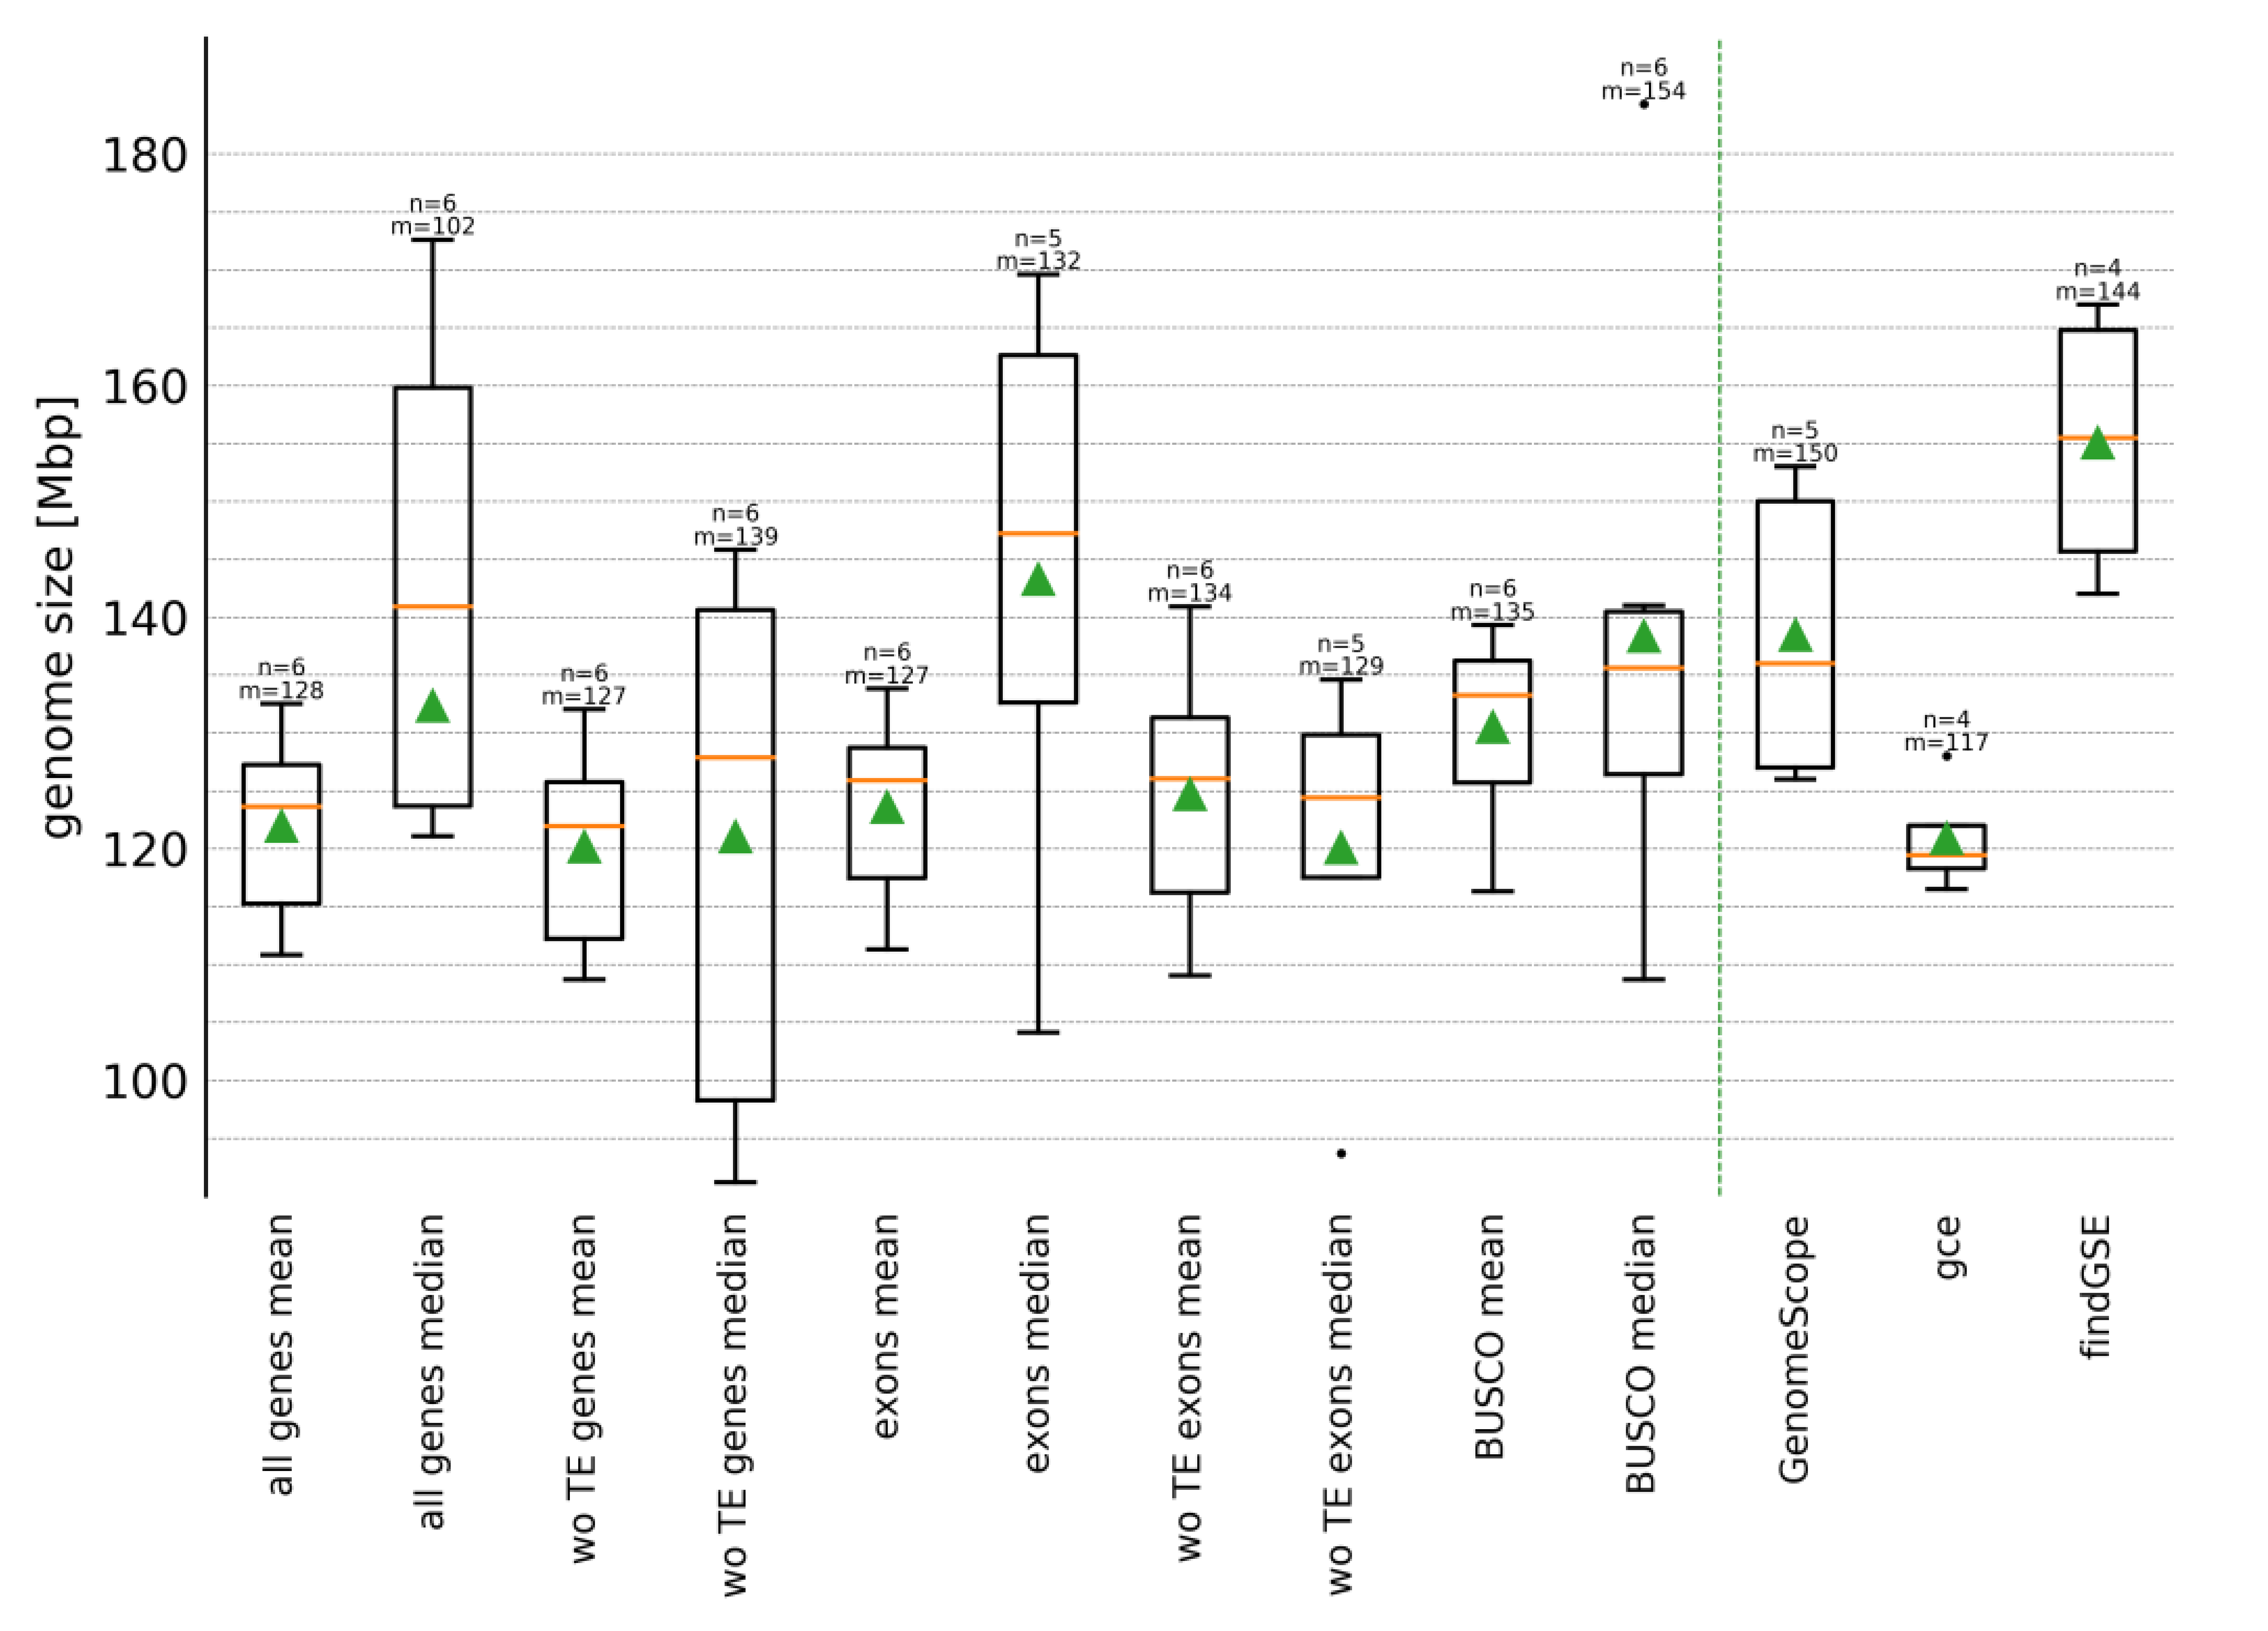
\includegraphics[width=0.7\textwidth]{capitoli/analisi/confronto/confronto2/1a.png}
		\caption{Dimensioni stimate dai metodi rispetto $n$ campioni di \gls{ecotipo} Col-0 di \textit{A. thaliana}. Per il metodo MGSE vengono scelte la media o la mediana di porzioni diverse di genoma. La figura mostra per ciascun metodo il valor medio (in verde) e la mediana $m$ (in giallo).}
		\label{fig:2confronto1a}
	\end{figure}
		
	Nell'analisi dell'\gls{ecotipo} Nd-1 mostrata dalla figura~\ref{fig:2confronto1b}, il metodo MGSE (sequenze BUSCO) mostra una differenza evidente nella stima della dimensione utilizzando la media o la mediana della copertura. Il valore stimato da MGSE attraverso la media delle sequenze BUSCO risulta il più affidabile, con una dimensione reale stimata di 138-140~Mb \cite{pucker2016denovo}. Mentre GCE restituisce un valore più plausibile, i metodi GenomeScope e findGSE generano una dimensione la cui correttezza risulta poco probabile.

	\begin{figure}[]
		\centering
		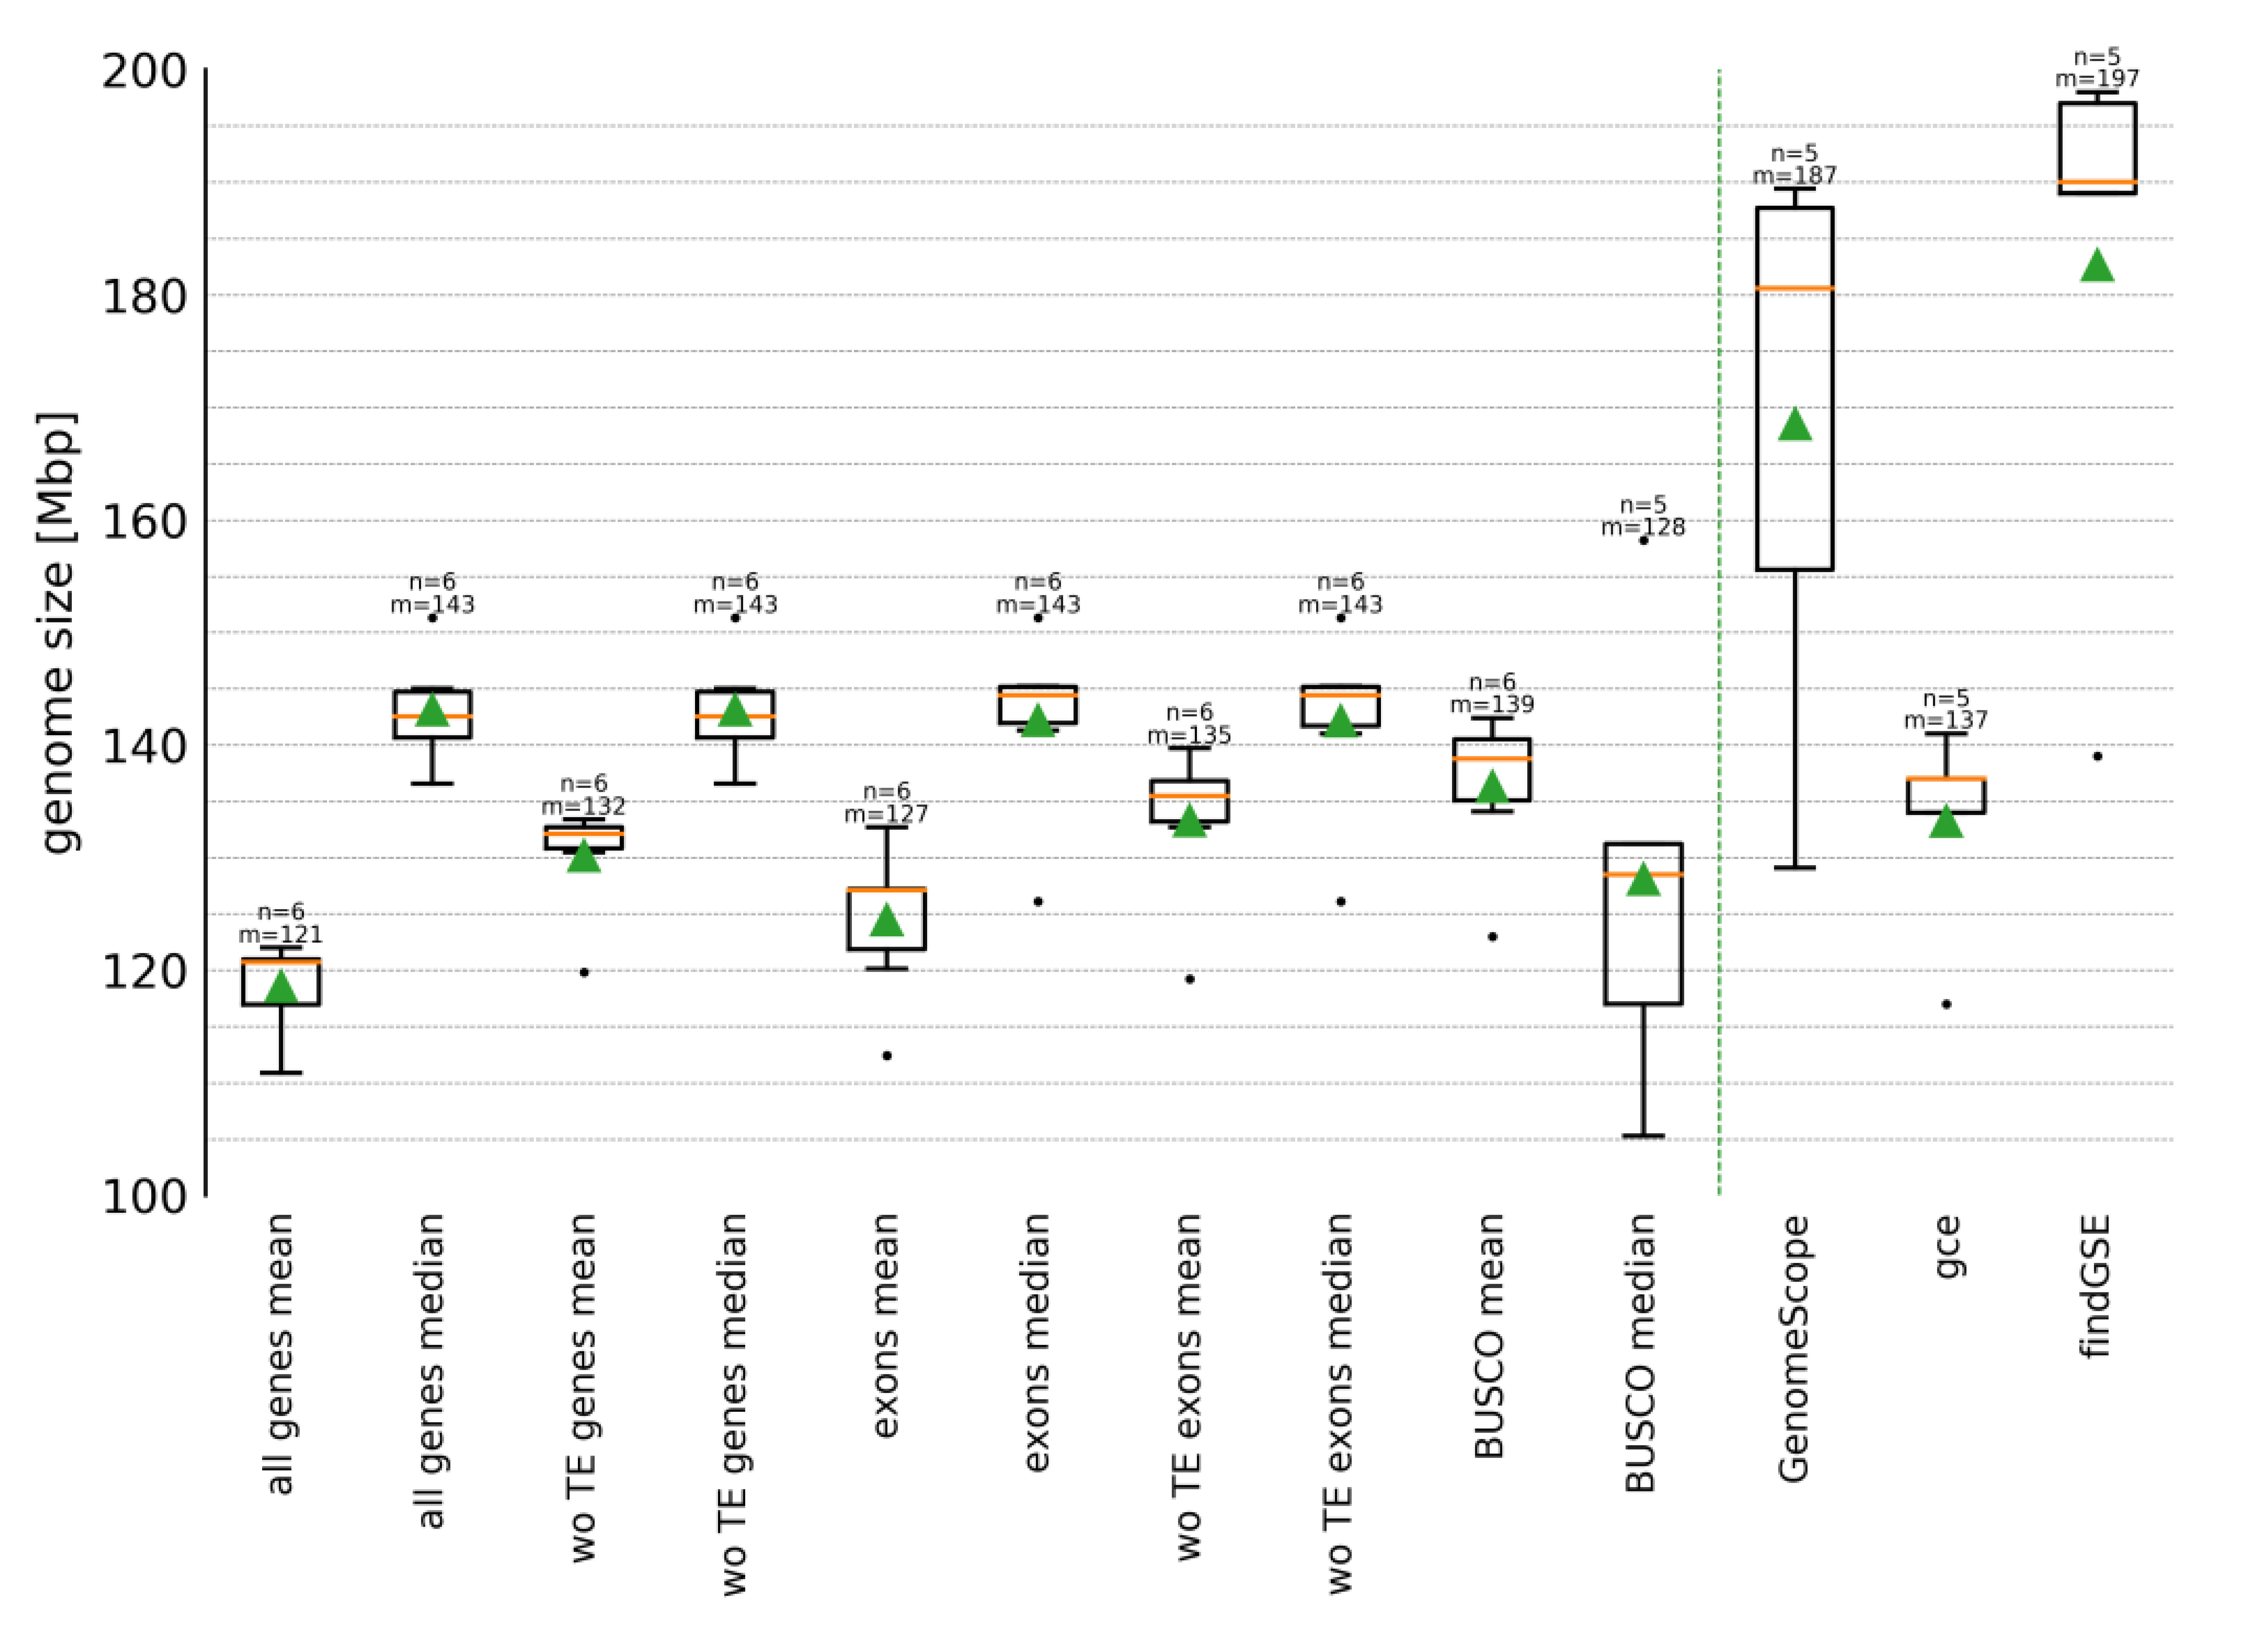
\includegraphics[width=0.7\textwidth]{capitoli/analisi/confronto/confronto2/1b.png}
		\caption{Dimensioni stimate dai metodi rispetto $n$ campioni di \gls{ecotipo} Nd-1 di \textit{A. thaliana}. Per il metodo MGSE vengono scelte la media o la mediana di porzioni diverse di genoma. La figura mostra per ciascun metodo il valor medio (in verde) e la mediana $m$ (in giallo).}
		\label{fig:2confronto1b}
	\end{figure}
	
	Il confronto prosegue quindi con la stima della dimensione del genoma a partire da 1028 sequenze di \textit{A. thaliana}. I programmi GCE, GenomeScope e findGSE nella maggior parte dei casi stimano valori compresi tra 120 e 200 Mb, mentre MGSE tra 120 e 160 Mb, come mostrato nella figura~\vref{fig:2confronto3}. Si riporta comunque che tutti i metodi hanno generano alcuni valori errati, estremamente elevati o ridotti. In media, findGSE tende a stimare valori maggiori rispetto agli altri metodi basati sui k-mer.
	
	\begin{figure}[]
		\centering
		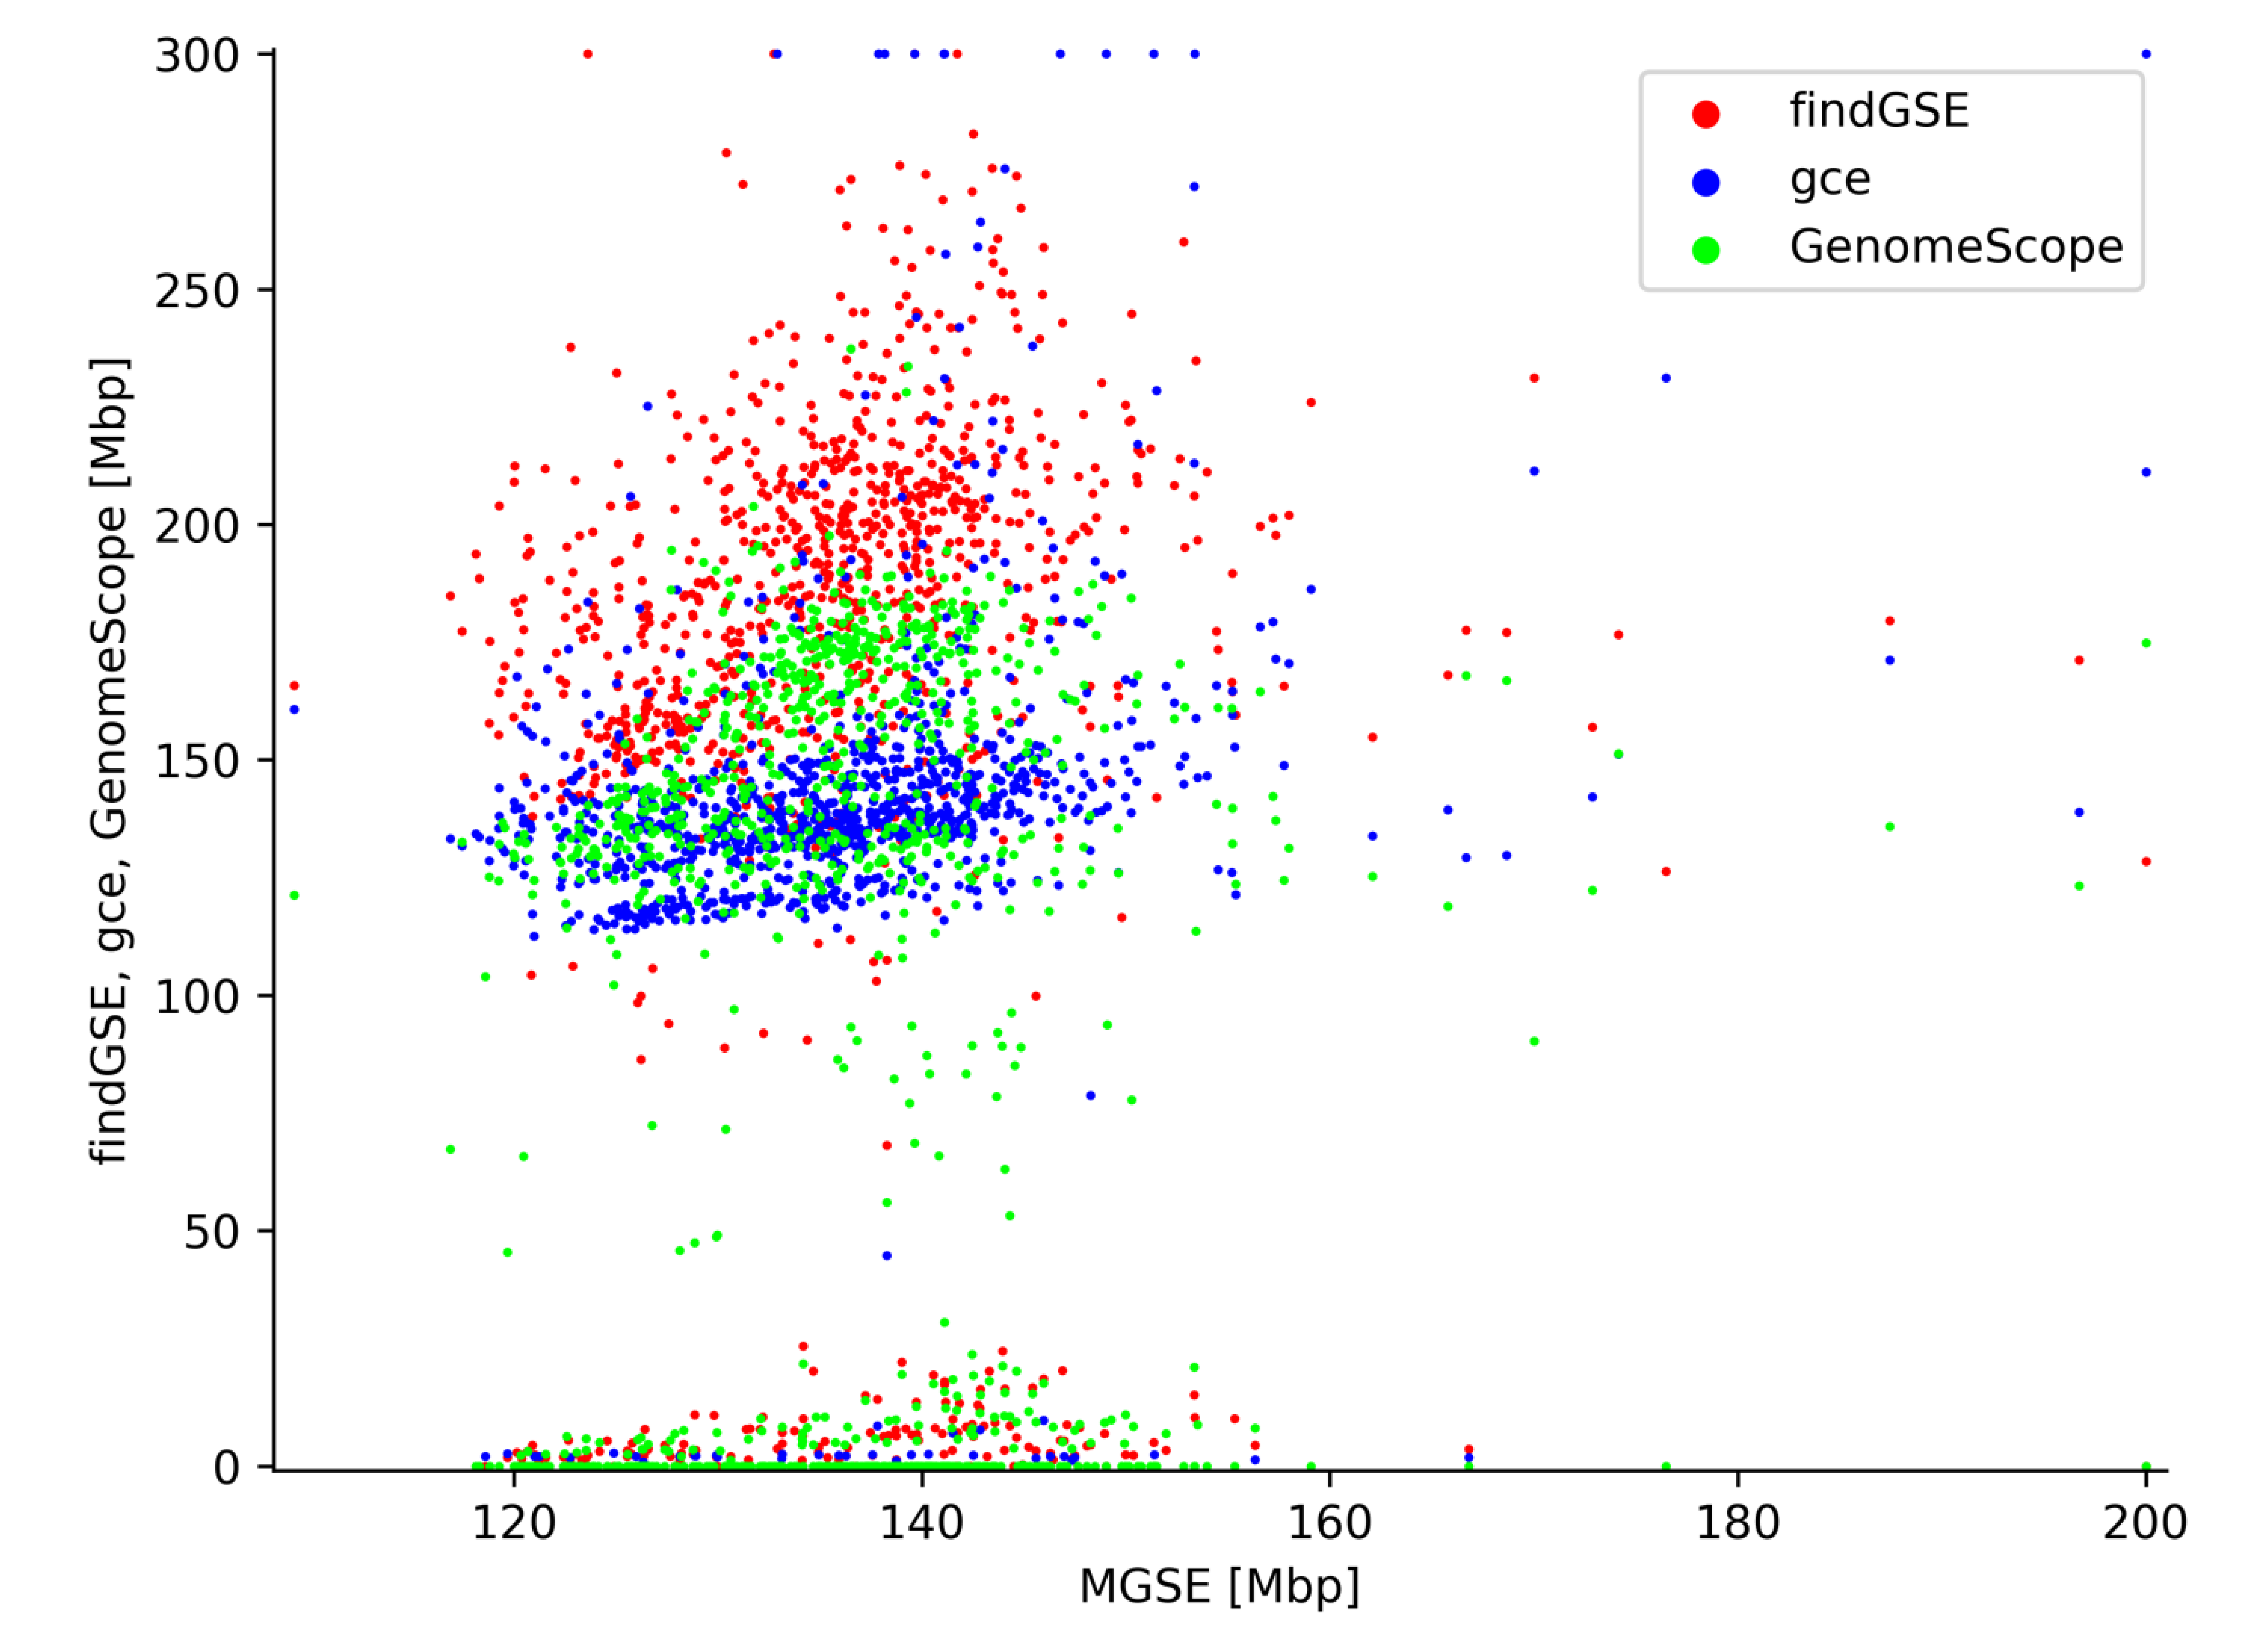
\includegraphics[width=0.7\textwidth]{capitoli/analisi/confronto/confronto2/2.png}
		\caption{Stima della dimensione di 1028 sequenze di \textit{A. thaliana}. I risultati dei metodi findGSE, GCE e GenomeScope vengono mostrati in funzione delle stime del metodo MGSE. Eventuali outlier vengono rappresentati sul bordo del grafico, permettendo una maggiore risoluzione alla nuvola centrale.}
		\label{fig:2confronto3}
	\end{figure} 

	\paragraph{Stima della dimensione di \textit{Beta vulgaris}}
	Per verificare l'accuratezza nella stima di genomi con maggiori dimensioni e complessità, i programmi vengono utilizzati per determinare la dimensione di \textit{Beta vulgaris}. Dato che vengono utilizzate sequenze diverse come dati iniziali, sono attese differenze minime tra le letture di input, che potrebbero far variare i valori stimati dai metodi. Comunque, dato che al momento del test l'assembly più sviluppato del genoma di tale specie comprende 567 Mb della sequenza completa, i valori minori di tale soglia possono essere classificati come erronei. 
	
	Come mostrato dalla figura~\vref{fig:2confronto4}, i metodi GenomeScope e GCE tendono a sottodimensionare la stima, restituendo valori in media di 500 Mb. Il programma findGSE, invece, genera risultati ad alta variabilità. Il metodo MGSE, utilizzando la media della copertura dei geni a singola copia o delle regioni BUSCO, sembra avere prestazioni migliori.
	
	\begin{figure}[]
		\centering
		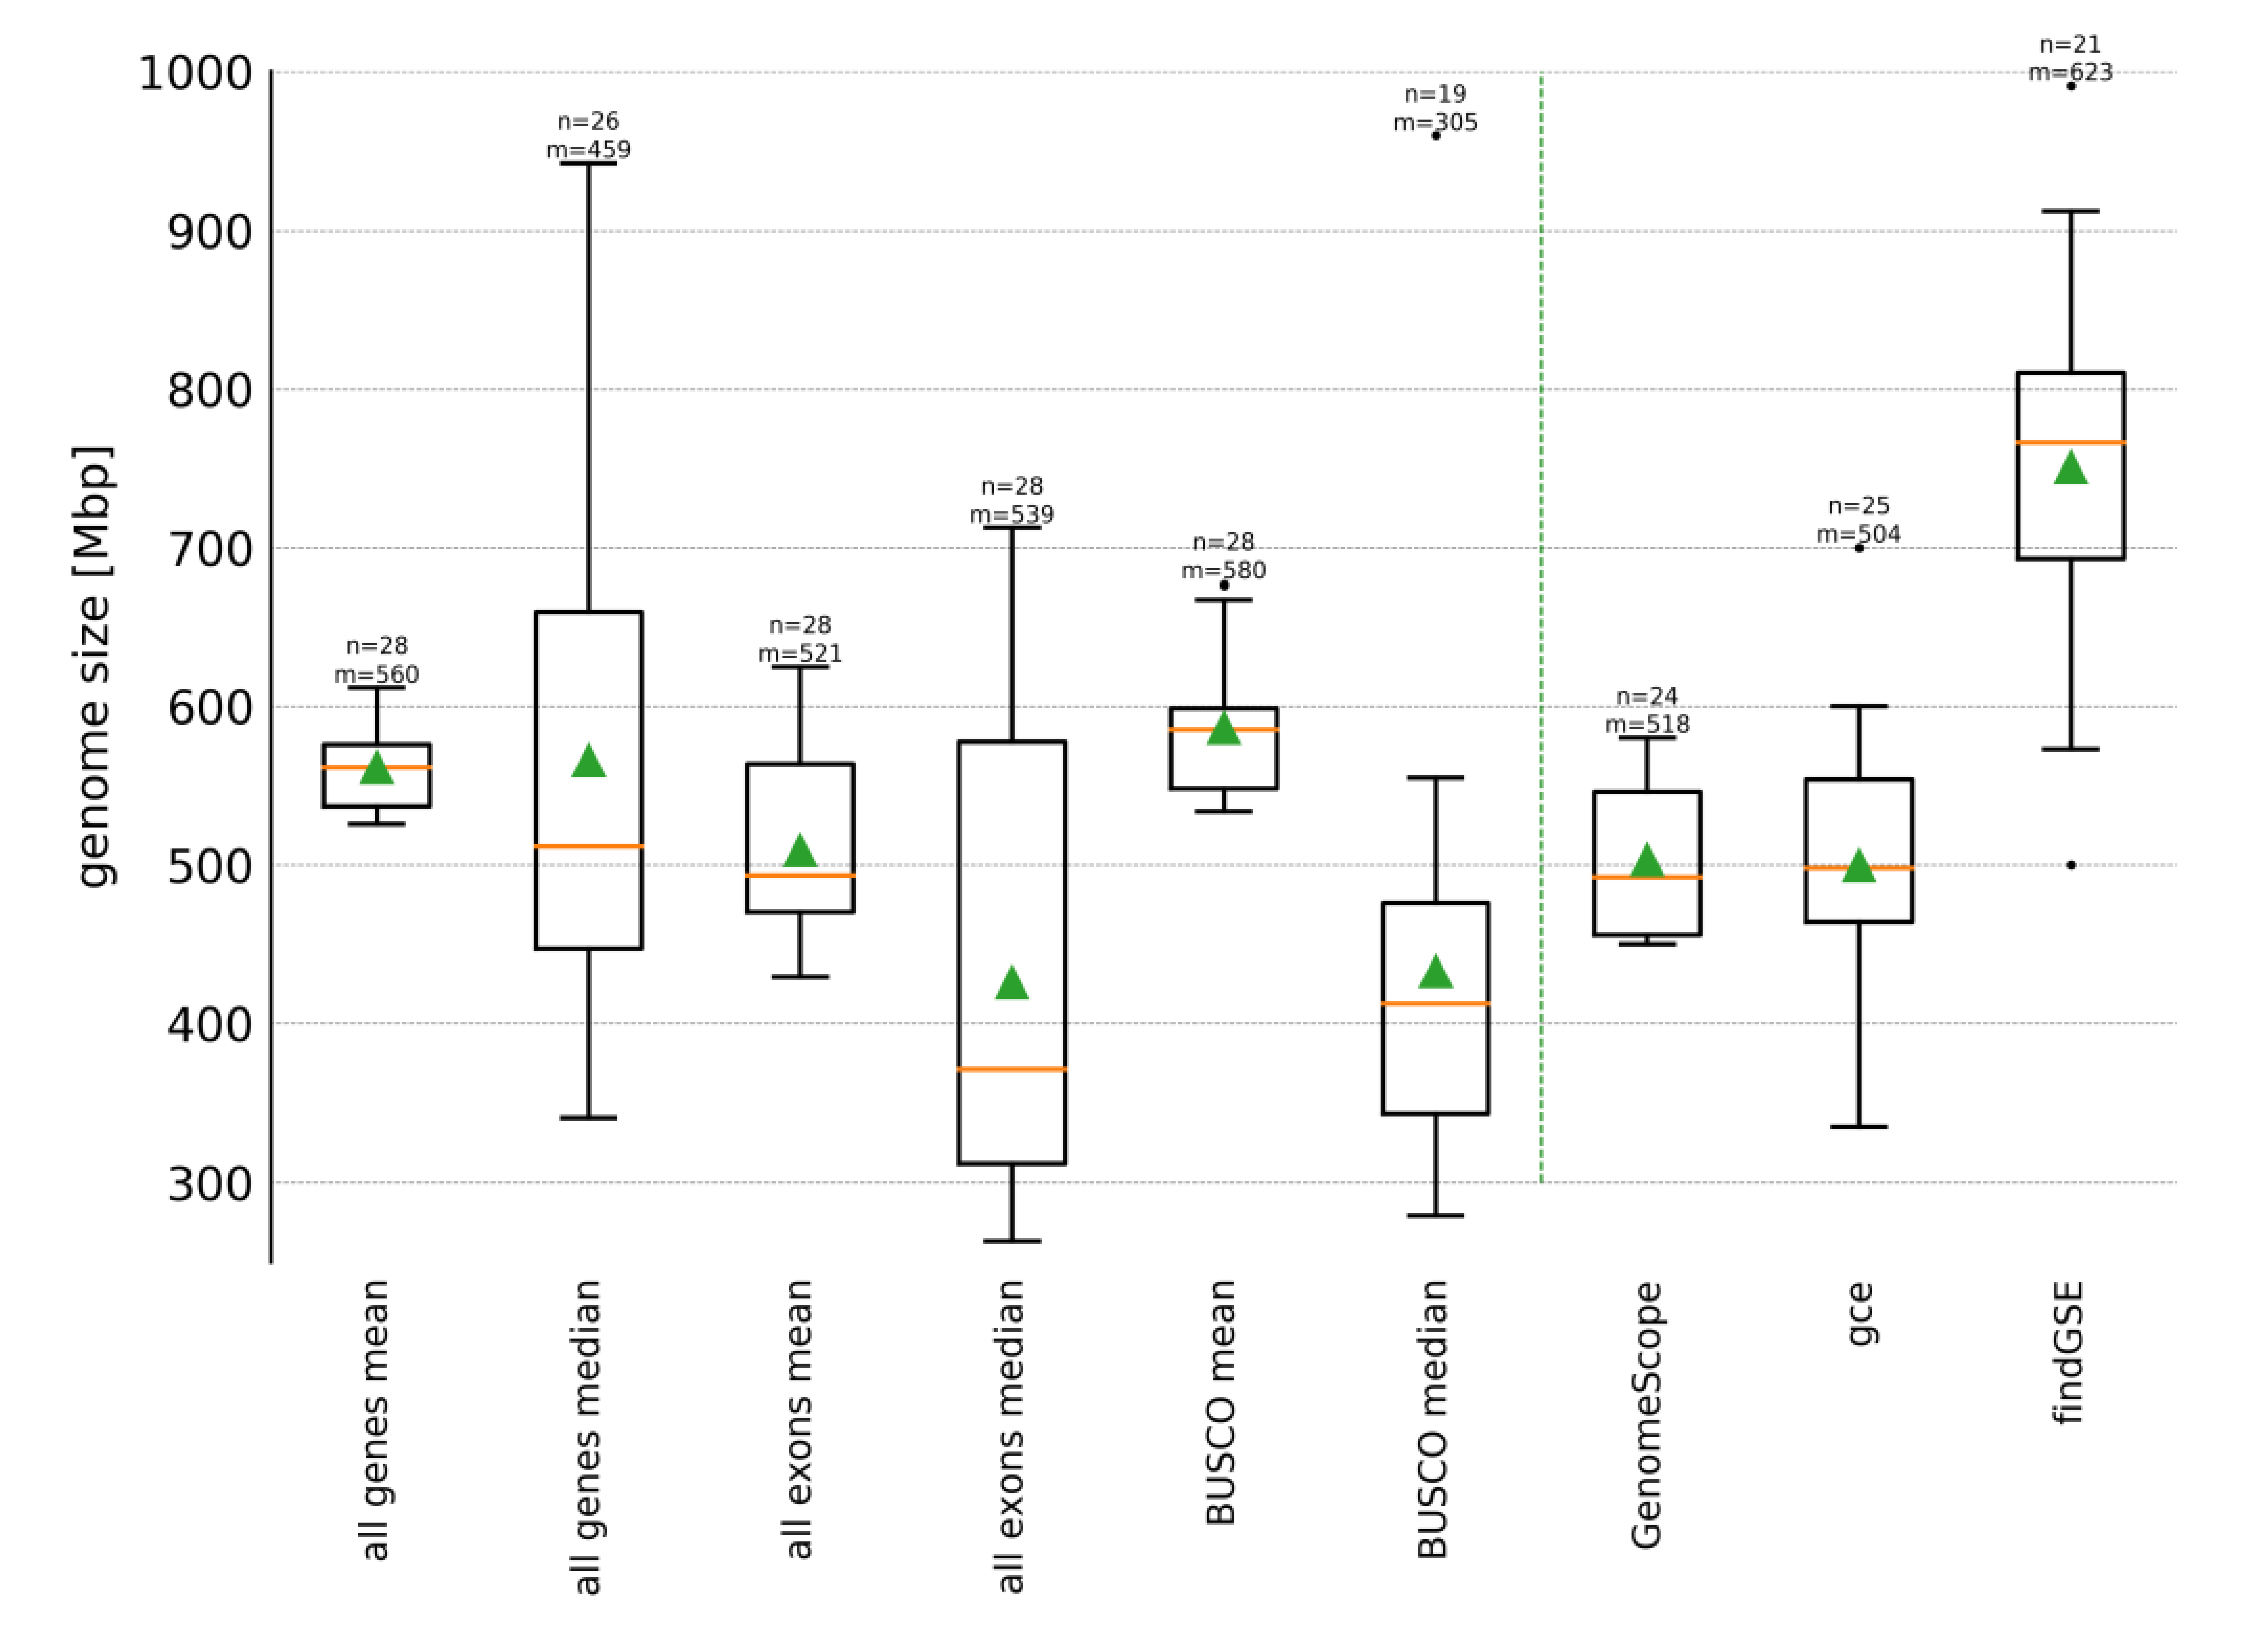
\includegraphics[width=0.7\textwidth]{capitoli/analisi/confronto/confronto2/3.png}
		\caption{Dimensioni stimate dai metodi rispetto $n$ campioni di \textit{Beta vulgaris}. Per il metodo MGSE vengono scelte la media o la mediana di porzioni diverse di genoma. La figura mostra per ciascun metodo il valor medio (in verde) e la mediana $m$ (in giallo).}
		\label{fig:2confronto4}
	\end{figure} 

	\paragraph{Dimensione di genomi di altre specie}
	L'analisi continua con la stima delle dimensioni di genomi di varie specie, ciascuna con caratteristiche diverse: il \textit{Brachypodium distachyon} come modello di pianta erbacea, il pomodoro (\textit{Solanum lycopersicum}) per il \gls{clade} delle Asteridi, il mais (\textit{Zea mays}) è stato incluso come specie monocotiledone ad alto contenuto di \glspl{trasposone}, e la vite comune (\textit{Vitis vinifera}) per la sua elevata eterozigosi.
	
	I programmi, come mostrato dalla figura~\vref{fig:2confronto5}, restituiscono generalmente risultati appartenenti al medesimo intervallo. Nella stima della dimensione di \textit{B. distachyon}, mentre MGSE, GenomeScope e GCE tendono a generare valori non corretti, findGSE stima una previsione ragionevole di 303 Mb, a fronte di una lunghezza stimata di circa 355 Mb \cite{ozdemir2008brachypodium}. 
	La dimensione del genoma di \textit{Z. mays} è ampiamente sottostimata da tutti i programmi, dato che la lunghezza stimata risulta di 2.4 Gb \cite{haberer2005structure}. 
	A differenza di MGSE e GCE, i programmi findGSE e GenomeScope stimano correttamente la lunghezza attesa di \textit{S. lycopersicum} (950 Mb \cite{barone2008structural}).	
	A causa dell'alta eterozigosi, MGSE restituisce un valore di soli 50 Mbp per il genoma di \textit{V. vinifera}, mentre il programma GenomeScope restituisce un valore plausibile, avendo una dimensione stimata di 475~Mb~\cite{myles2010rapid}.

	\begin{figure}
		\centering
		\subfloat[][\emph{Stima della dimensione del genoma di specie \textit{Brachypodium distachyon}.}]
			{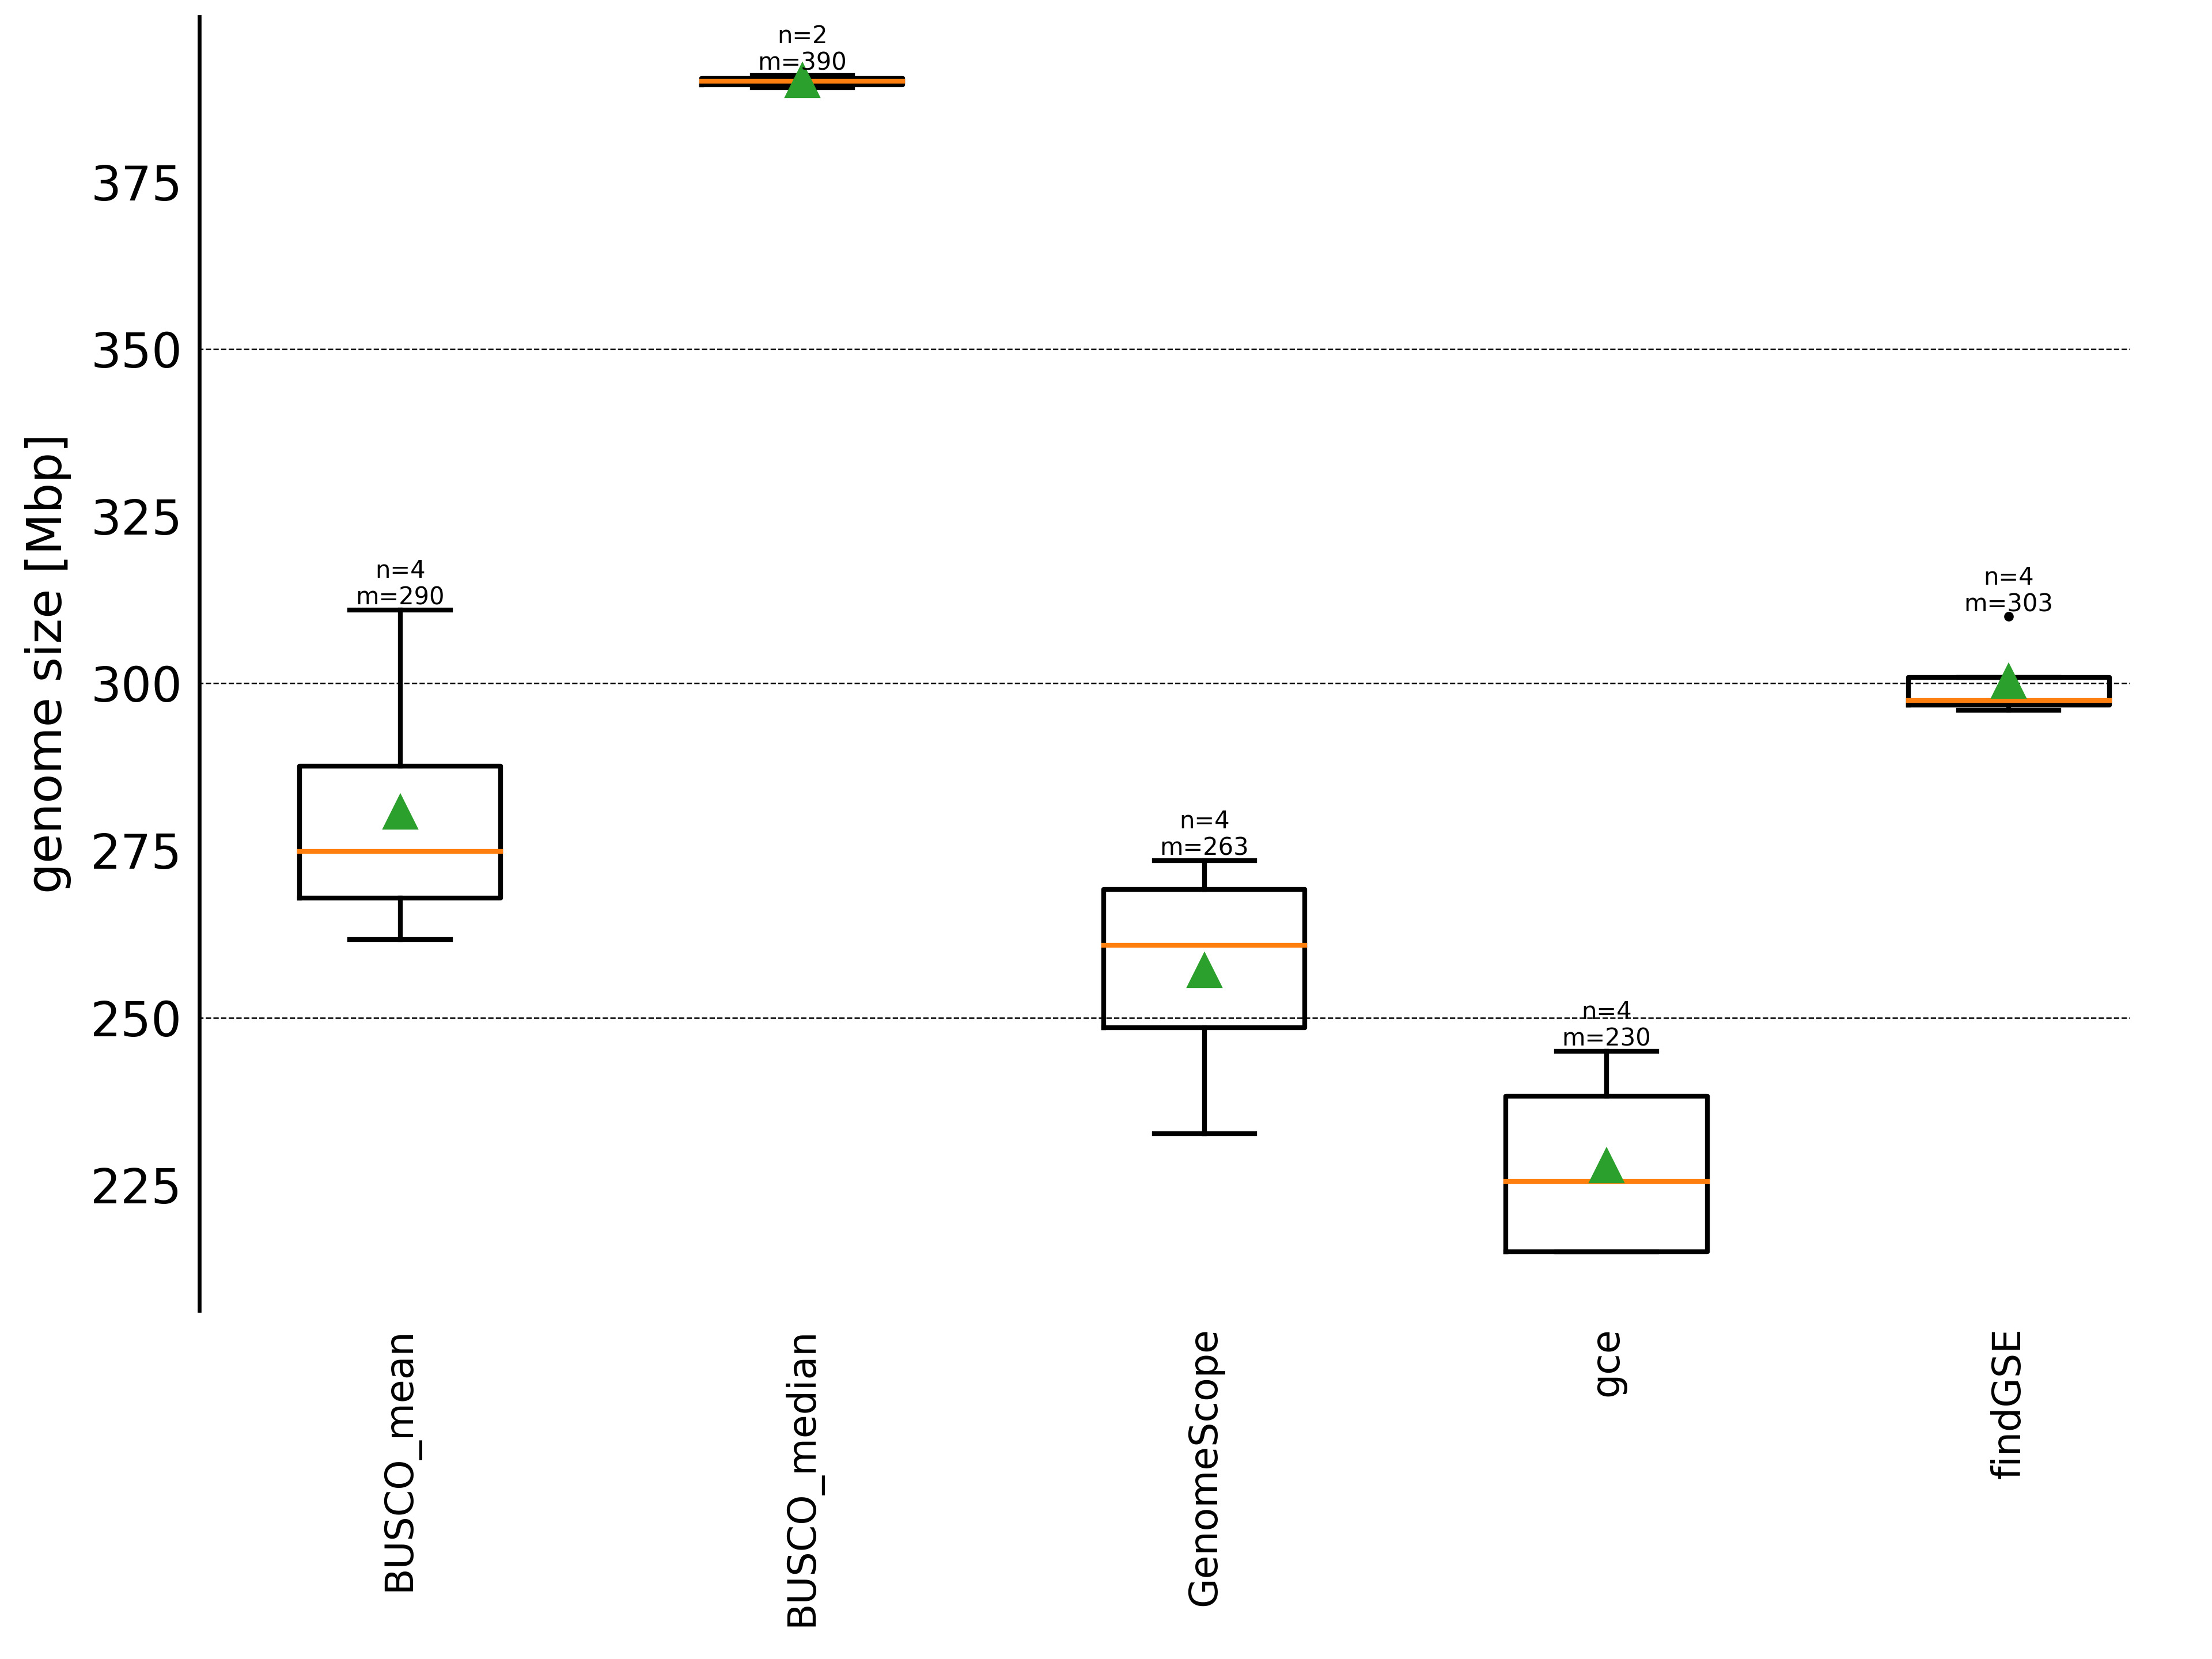
\includegraphics[width=0.45\textwidth]{capitoli/analisi/confronto/confronto2/6.jpg}} \quad
		\subfloat[][\emph{Stima della dimensione del genoma di specie \textit{Zea mays}.}]
			{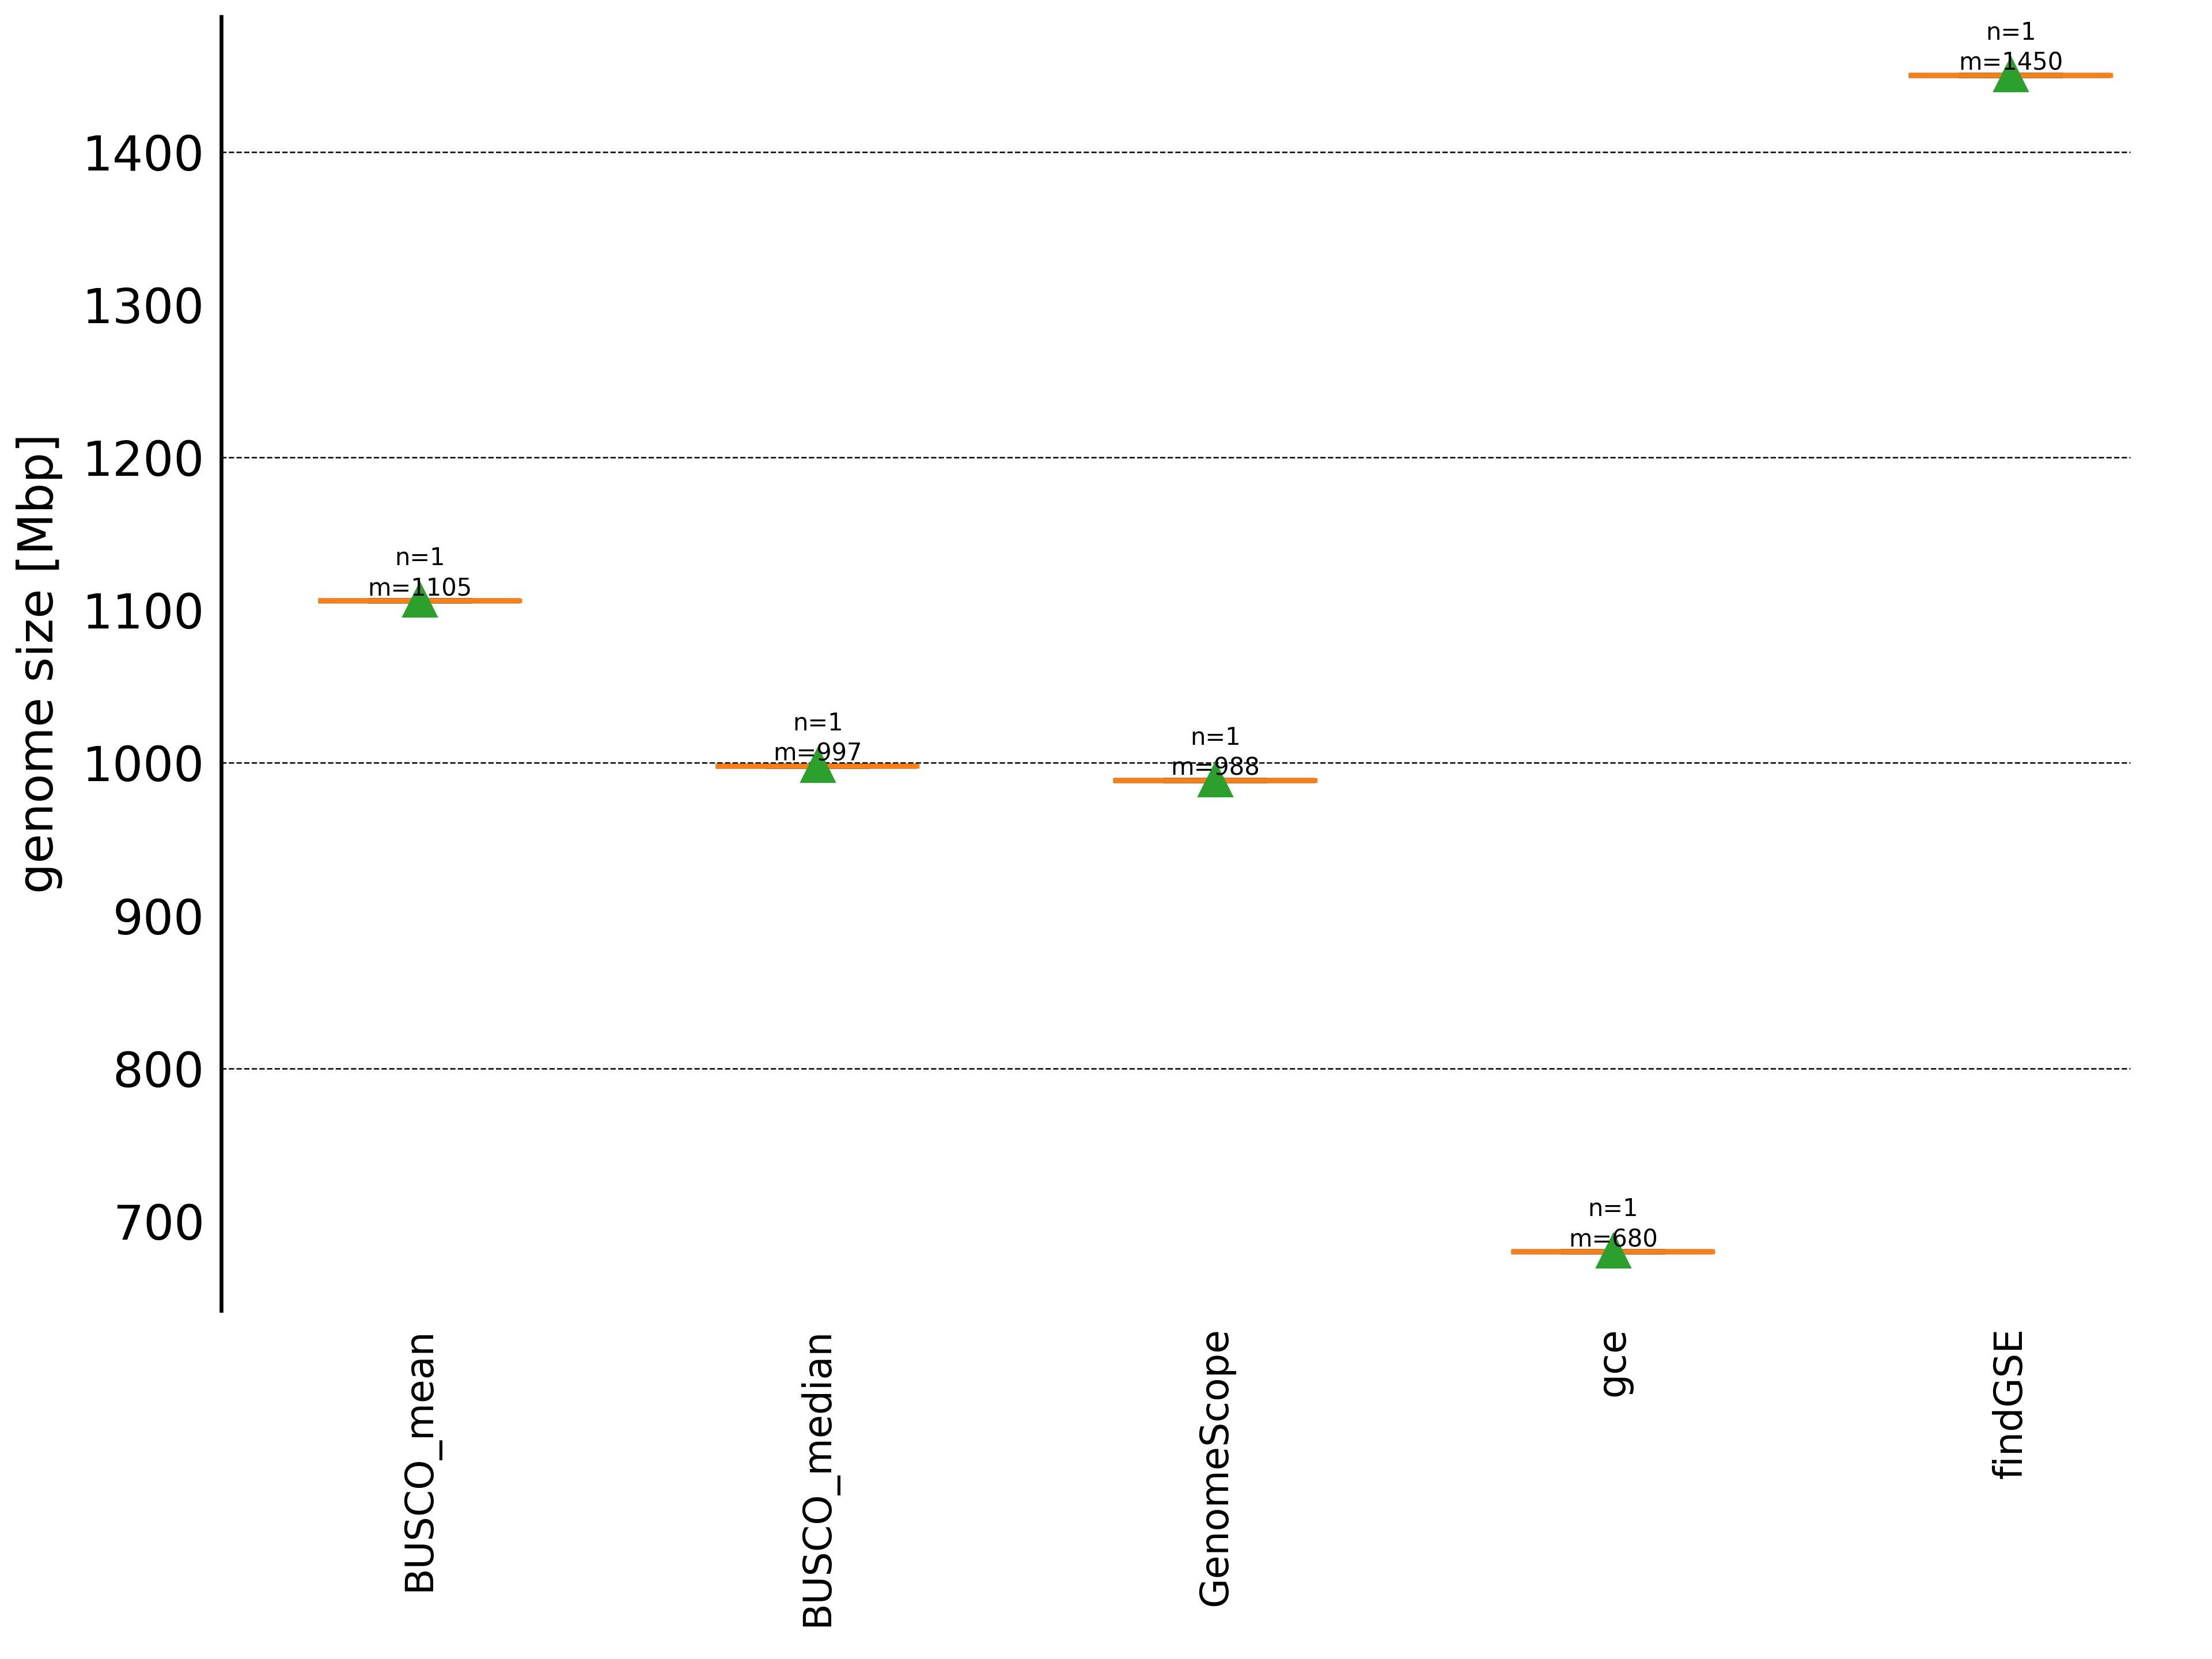
\includegraphics[width=0.45\textwidth]{capitoli/analisi/confronto/confronto2/7.jpg}} \\ 
		\subfloat[][\emph{Stima della dimensione del genoma di specie \textit{Solanum lycopersicum}.}]
			{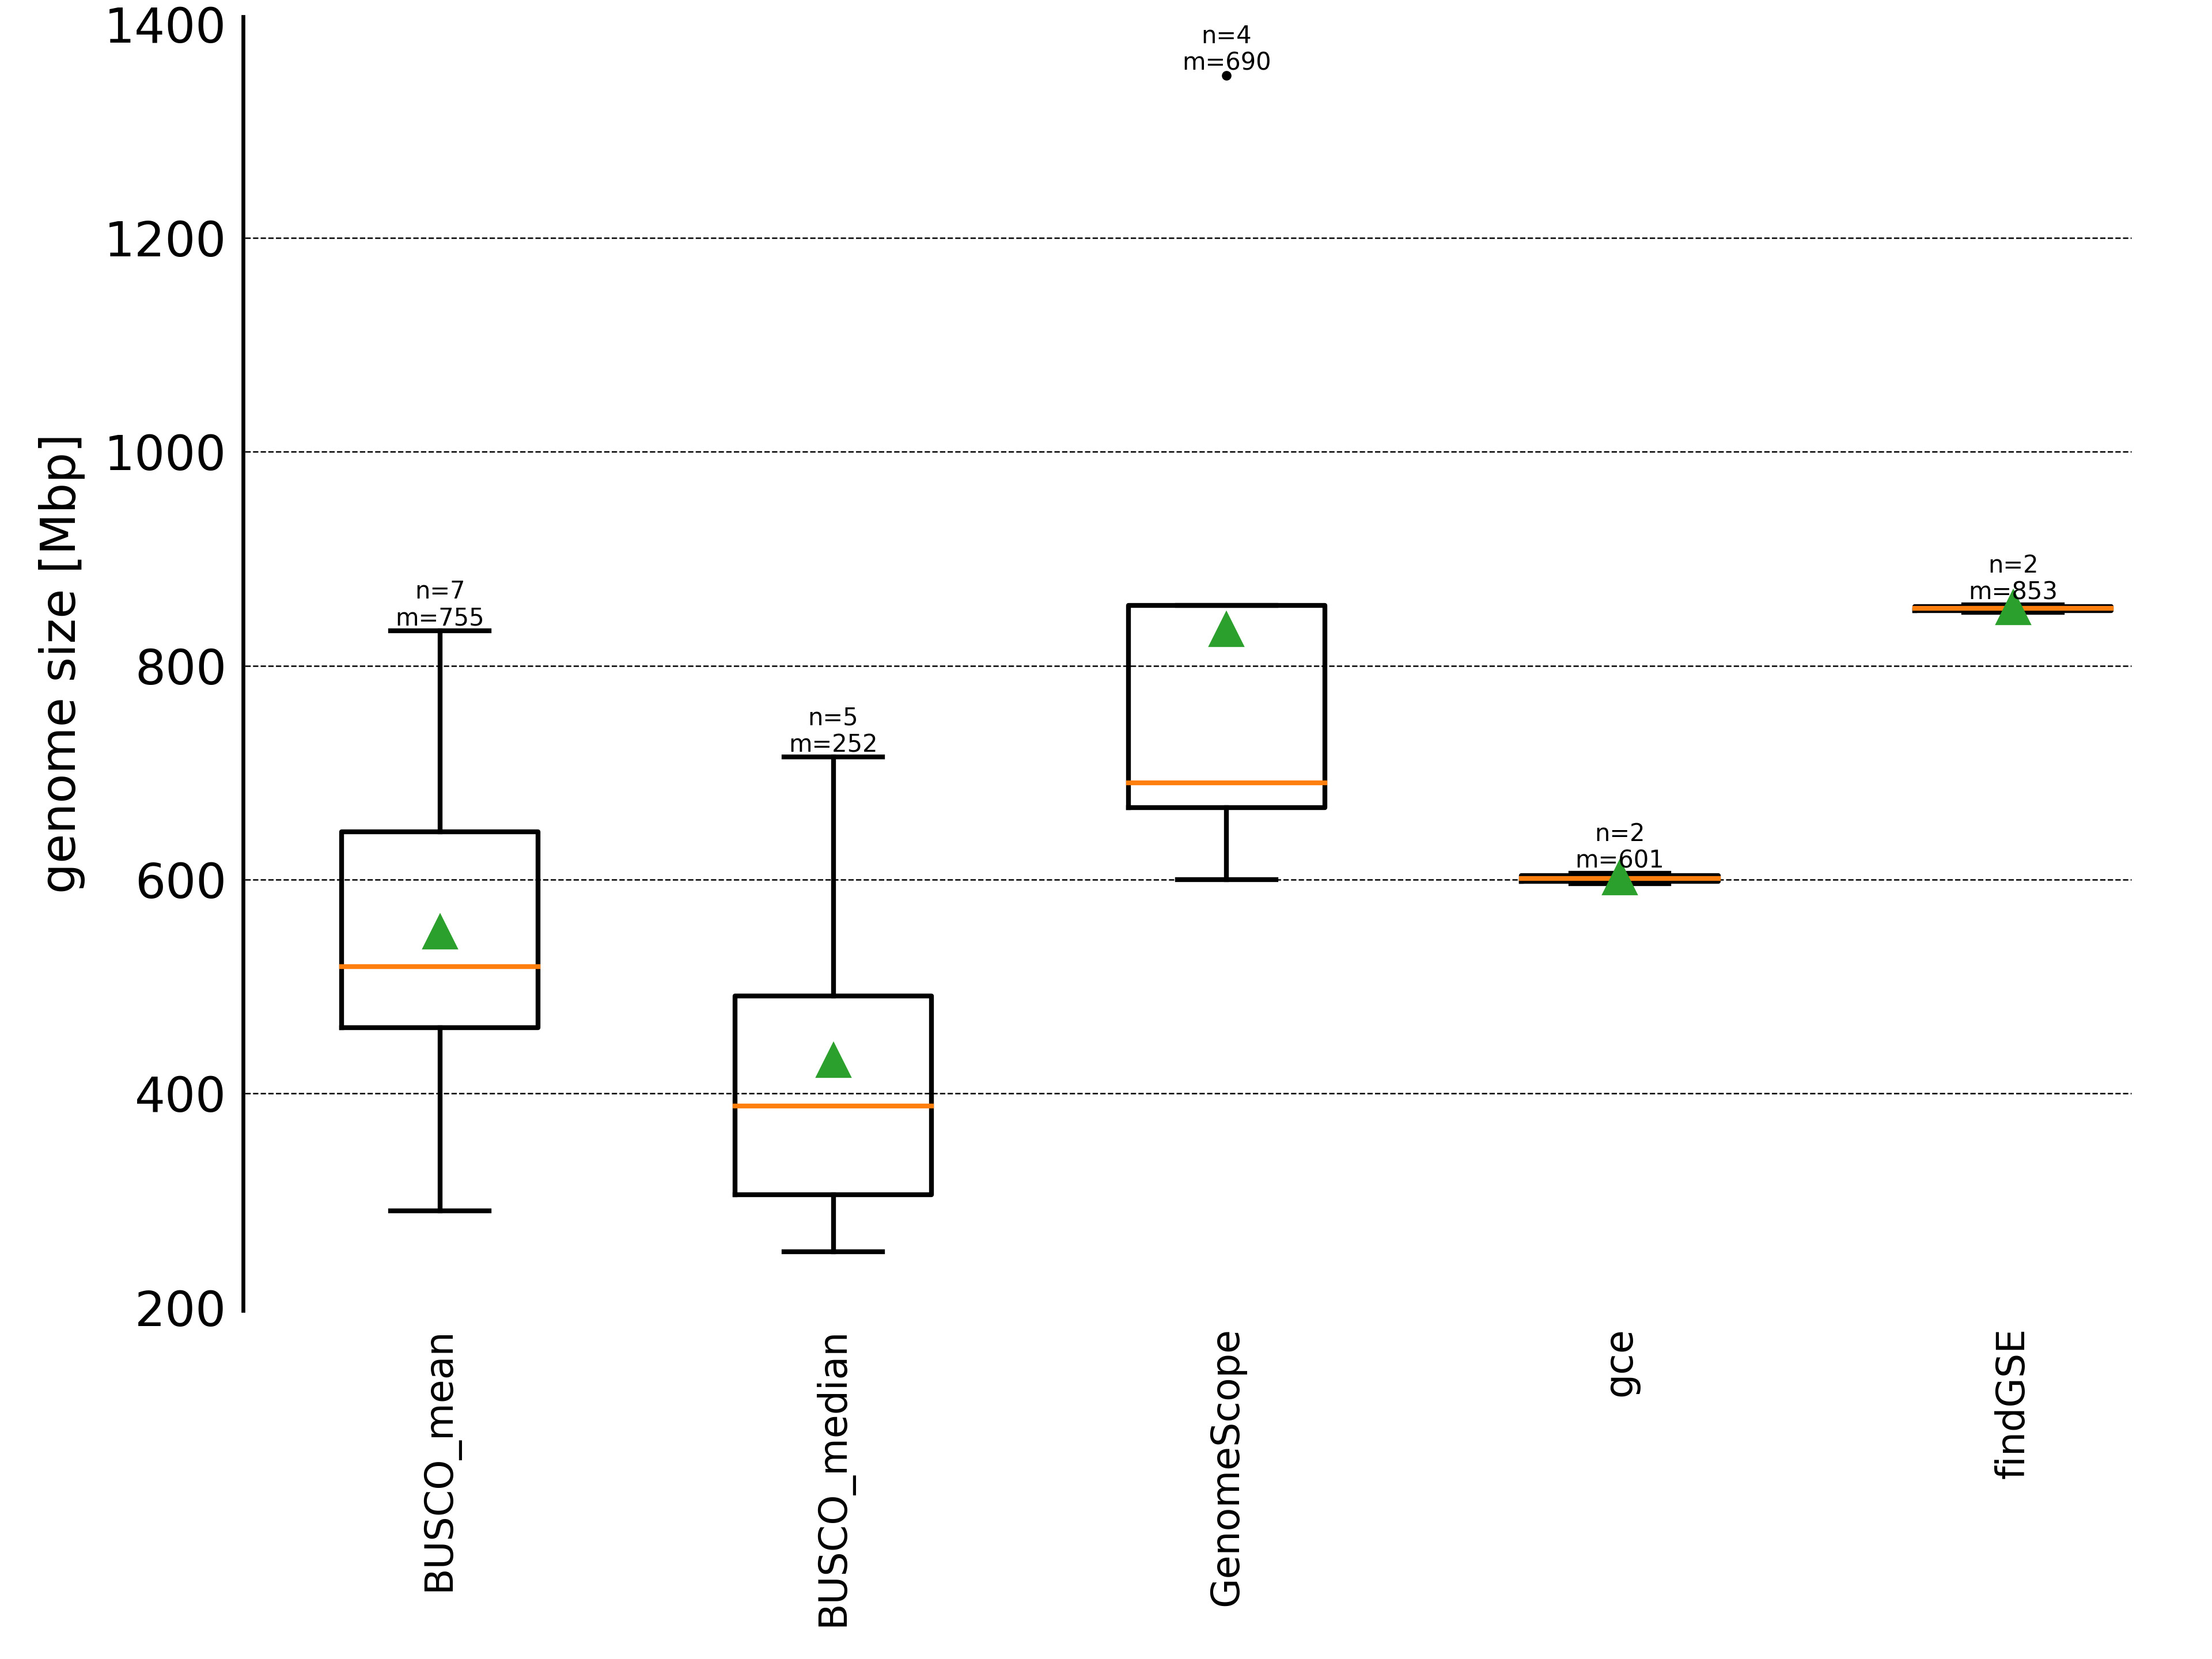
\includegraphics[width=0.45\textwidth]{capitoli/analisi/confronto/confronto2/8.jpg}} \quad
		\subfloat[][\emph{Stima della dimensione del genoma di specie \textit{Vitis vinifera}.}]
			{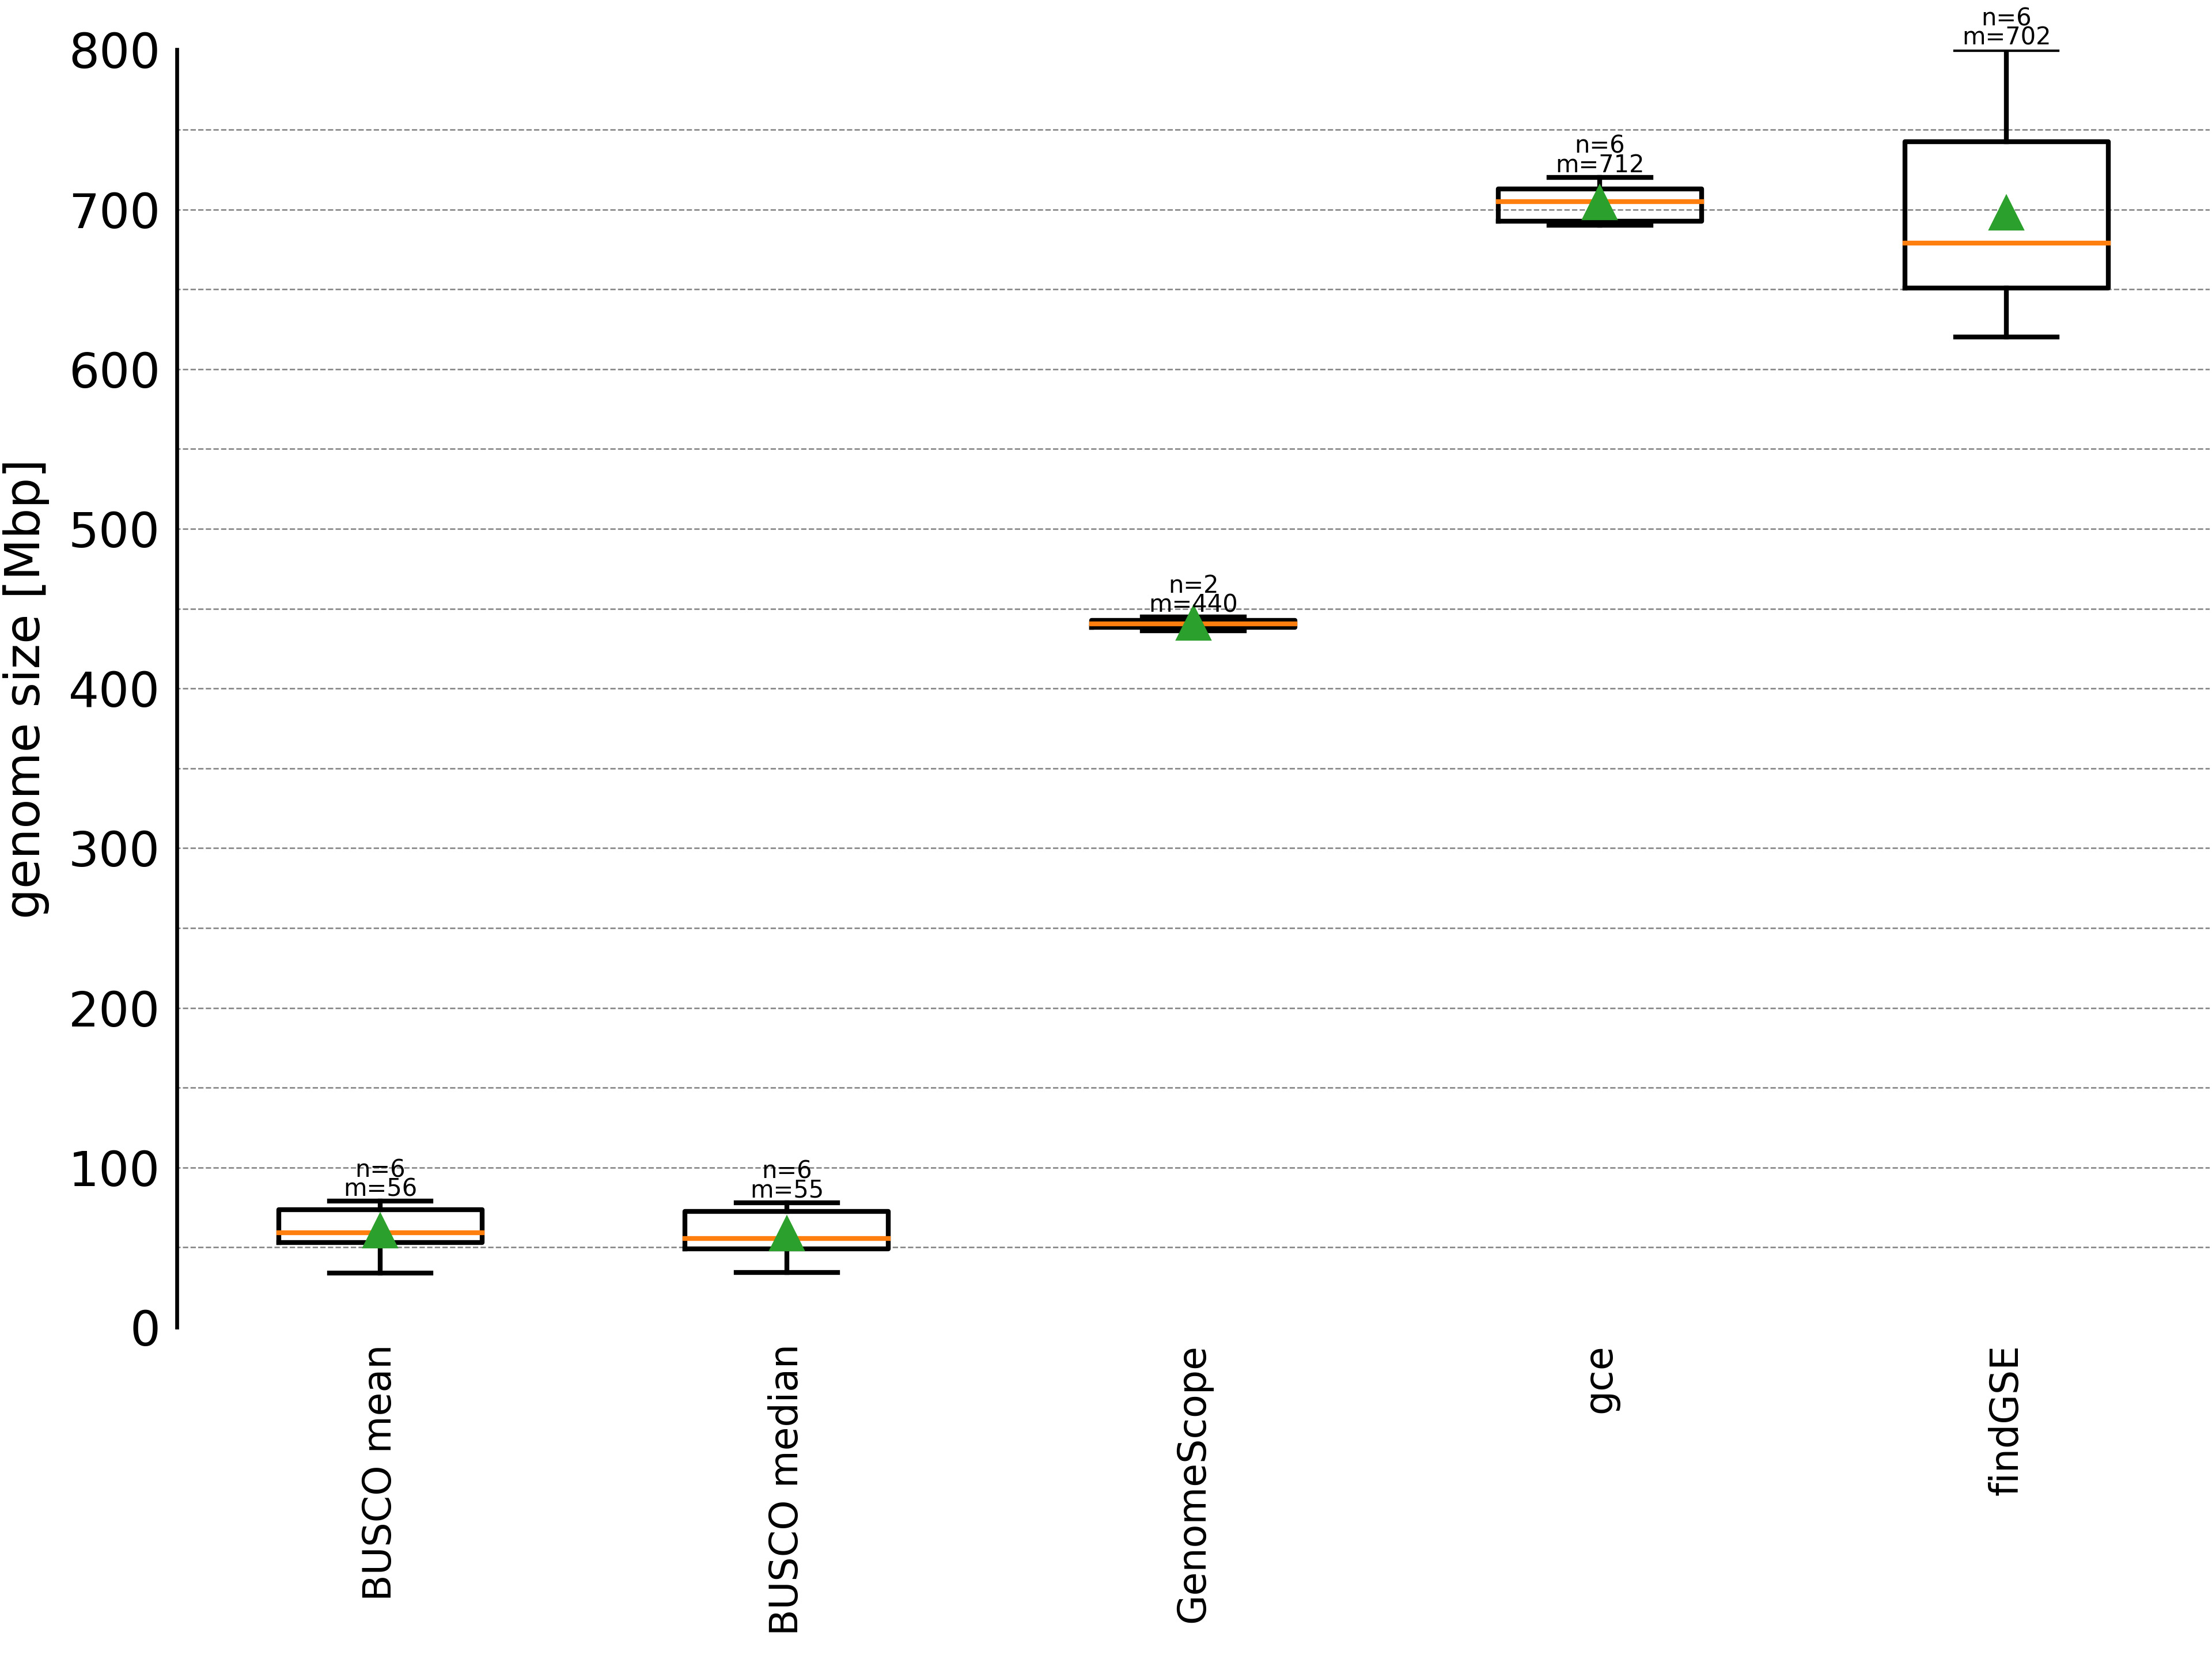
\includegraphics[width=0.45\textwidth]{capitoli/analisi/confronto/confronto2/9.jpg}}
		\caption{Dimensioni stimate dai metodi rispetto $n$ campioni di genomi di varie specie. Per il metodo MGSE vengono scelte la media o la mediana delle regioni BUSCO. La figura mostra per ogni stima il valor medio (in verde) e la mediana $m$ (in giallo).}
		\label{fig:2confronto5}
	\end{figure}
\end{document}